\DiaryEntry{Predator-Prey (Lotka-Volterra Equations)}{2024-06-05}{Maths}

Based on entry \ref{2018-07-30:entry} and extended to general coefficients here. We consider the following ODE system,

\begin{align}\label{2024-06-05-eq1}
R' = \frac{dR}{dt} &= \alpha R - \beta RF \nonumber \\
F' = \frac{dF}{dt} &= -\gamma F + \delta RF
\end{align}

We can rewrite the first equation as $R(\alpha - \beta F) = 0$ and obtain two fixed points from it: (i) $R = $, (ii) $F = \alpha/\beta$. We can use the second equation similarly, $F(- \gamma+  \delta R)$ and obtain (i) $F = 0$, (ii) $R = \gamma/\delta$. Therefore, we have two fixed points,

\begin{align}
  &R = F = 0\\
  &R = \gamma / \delta, F = \alpha / \beta
\end{align}

To assess the stability of the fixed points, we calculate the Jacobian $\Jbf$ of the differential equation system,

\bee
\Jbf = \begin{pmatrix} \frac{dR'}{dR} & \frac{dR'}{dF} \\ \frac{dF'}{dR} & \frac{dF'}{dF} \end{pmatrix} = \begin{pmatrix} \alpha - \beta F & - \beta R \\ \delta F & \delta R - \gamma \end{pmatrix}
\eee

Let's consider the fixed point $R = F = 0$ first. For these values, the Jacobian becomes

\bee
\Jbf_1 = \begin{pmatrix} \alpha & 0 \\ 0 & - \gamma \end{pmatrix}
\eee

The eigenvalues are the solution to $|\Jbf_1 - \lambda \Ibf | = 0$. We have

\bee
\begin{vmatrix} \alpha - \lambda & 0 \\ 0 & - \gamma - \lambda \end{vmatrix} = (\alpha - \lambda)(- \gamma - \lambda) = 0
\eee

and therefore the two eigenvalues become $\lambda_1 = \alpha, \lambda_2 = - \gamma$. In our model, the parameters $\alpha$ and $\gamma$ are always greater than zero, and therefore the sign of the eigenvalues will be different. Hence the fixed point at the origin is a saddle point which is an instable fixed point. Depending on the starting point, the solution will either reach the fixed point $R = F = 0$ or diverge away from it. The first case happens for all starting points $R=0, F > 0$: The foxes do not find find food and therefore die out.

This is show in the following population plot.

\begin{figure}[H]
    \centering
    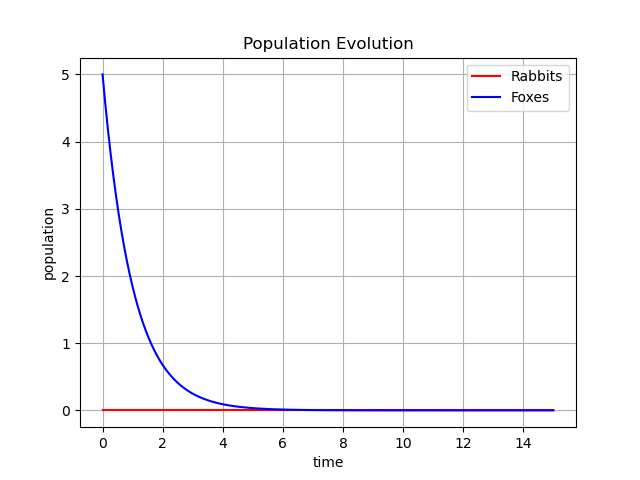
\includegraphics[scale=0.75]{images/2024-06-05-pred_prey_01.png}
\end{figure}


The second case happens for all starting points $R>0, F=0$: There are no enemies for the rabbits and therefore they grow unlimited.

This is show in the following population plot.

\begin{figure}[H]
    \centering
    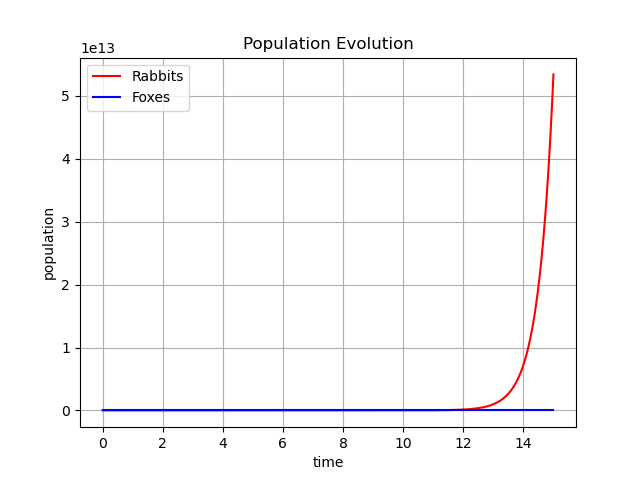
\includegraphics[scale=0.75]{images/2024-06-05-pred_prey_02.png}
\end{figure}


For the other fixed point ($R = \gamma / \delta, F = \alpha / \beta$), the Jacobian becomes

\bee
\Jbf_2 = \begin{pmatrix} \alpha - \beta \alpha / \beta & - \beta \gamma / \delta \\ \delta \alpha / \beta & \delta \gamma / \delta - \gamma \end{pmatrix} = \begin{pmatrix} 0 & - \beta \gamma / \delta \\ \delta \alpha / \beta & 0 \end{pmatrix}
\eee

The eigenvalues of this matrix are given by

\bee
\begin{vmatrix} -\lambda & - \beta \gamma / \delta \\ \delta \alpha / \beta & - \lambda \end{vmatrix} = \lambda^2 - (- \beta \gamma / \delta)(\delta \alpha / \beta) = 0
\eee

From this follows

\bee
\lambda^2 + \alpha \gamma = 0 \rightarrow \lambda_{1,2} = \pm j \sqrt{\alpha \gamma}
\eee

As the eigenvalues are both purely imaginary and conjugate to each other, this fixed point must either be a center for closed orbits in the local vicinity or an attractive or repulsive spiral. In conservative systems, there must be closed orbits in the local vicinity of fixed points, so we have a periodic solution.

An example for such a solution is shown in the following Figure ($\alpha=2, \beta=1, \gamma=1, \delta=1/3$).

\begin{figure}[H]
    \centering
    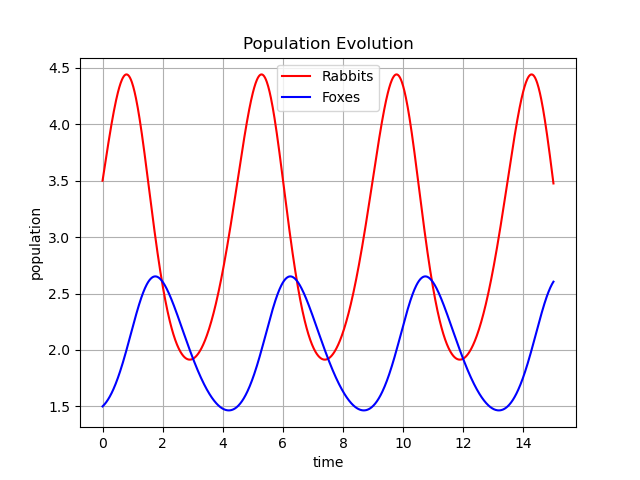
\includegraphics[scale=0.75]{images/2024-06-05-pred_prey_10.png}
\end{figure}

To illustrate the different behaviour we finally show the phase plot of the ODE system (same parameters as above). The fixed point is at $R = \gamma / \delta = 3, F = \alpha / \beta = 2$ and the ellipses are centered around this point. We can also see that in the population plots in the Figure above.

\begin{figure}[H]
    \centering
    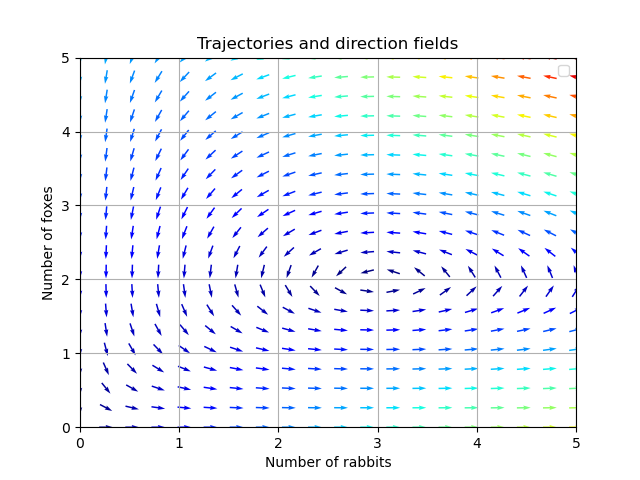
\includegraphics[scale=0.75]{images/2024-06-05-pred_prey_11.png}
\end{figure}

\subsection{ODE Linearization}

We want to linearize the ODE system around the second fixed point $R_0 = \gamma / \delta, F_0 = \alpha / \beta$. To this end we split off pertubation $r$ and $f$ around the fixed point,

\begin{align*}
    R &= R_0 + r = \gamma / \delta + r \\
    F &= F_0 + f = \alpha / \beta + r
\end{align*}

The derivatives in \eqref{2024-06-05-eq1} therefore become

\bee
R' = r' = \alpha R - \beta RF = \alpha \left(\frac{\gamma}{\delta} + r\right)- \beta \left(\frac{\gamma}{\delta} + r \right) \left( \frac{\alpha}{\beta} + f\right)
\eee

and we further obtain

\begin{align*}
    r' &= \alpha \left(\frac{\gamma}{\delta} + r \right)- \beta \left(\frac{\gamma}{\delta} \frac{\alpha}{\beta} + r \frac{\alpha}{\beta} + f \frac{\gamma}{\delta} + rf\right)\\
    &= \alpha \frac{\gamma}{\delta} + \alpha r  - \alpha \frac{\gamma}{\delta}  - r \alpha - f \frac{\beta \gamma}{\delta} - \beta rf \\
    &= - f \frac{\beta \gamma}{\delta} - \beta rf 
\end{align*}

For small pertubations around the fixed point, the product $rf$ will be small and is neglected for the linearization. We therefore have

\be\label{2024-06-05-eq2}
r' \approx - f \frac{\beta \gamma}{\delta}
\ee

In a similar spirit, we perform the same steps for $f'$

\begin{align*}
    F' &= f' = -\gamma F + \delta RF = -\gamma \left( \frac{\alpha}{\beta} + f \right) + \delta \left( \frac{\gamma}{\delta} + r\right) \left( \frac{\alpha}{\beta} + f\right) \\
    &= -\gamma \frac{\alpha}{\beta} - \gamma f + \delta \left( \frac{\gamma}{\delta} \frac{\alpha}{\beta} + r \frac{\alpha}{\beta} + f \frac{\gamma}{\delta} + rf \right) \\
    &= -\gamma \frac{\alpha}{\beta} - \gamma f + \frac{\alpha \gamma}{\beta} + r \frac{\delta \alpha}{\beta} + f \gamma + \delta rf \\
    &=  r \frac{\delta \alpha}{\beta} + \delta rf
\end{align*}

Making the linear approximation, we obtain

\be\label{2024-06-05-eq3}
f' \approx  r \frac{\delta \alpha}{\beta}
\ee

Combining \eqref{2024-06-05-eq2} and \eqref{2024-06-05-eq3}, we have the following linearized system

\begin{align*}
    r' &\approx - f \frac{\beta \gamma}{\delta} \\
    f' &\approx  r \frac{\delta \alpha}{\beta}
\end{align*}

We can convert this into a second order ODE by differentiating the first equation (and omitting the approximation signs)

\bee
    r'' = - \frac{\beta \gamma}{\delta} f'
\eee

Inserting the second equation yields

\bee
    r'' = - \frac{\beta \gamma}{\delta} \frac{\delta \alpha}{\beta} r = - \alpha \gamma r \rightarrow r'' + \alpha \gamma r = 0
\eee

This is a second order ODE of the form $r'' + r \alpha \gamma = 0$ and as we all know, this has solutions of the form $r(t) = C_1 \cos(\omega t) + C_2 \sin(\omega t)$ with $\omega = \alpha \gamma$. In our case we have $\omega \approx 0.816$ and therefore the periodicity is $T = 2 \pi \omega \approx 5.13$. The Figure below shows the two populations over time and also the approximately scaled and shifted linearized solution.

\begin{figure}[H]
    \centering
    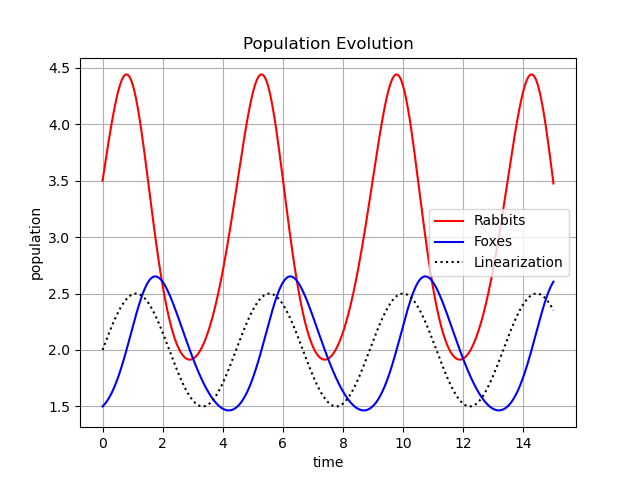
\includegraphics[scale=0.75]{images/2024-06-05-pred_prey_20.png}
\end{figure}

We finally note that the linear approximation holds well for initial points near the fixed point (shown in the left Subfigure below) and gets worse the further away the initial point from the fixed point is (shown in the right Subfigure below).

\begin{figure}[H]
    \begin{subfigure}{0.5\textwidth}
        \centering
        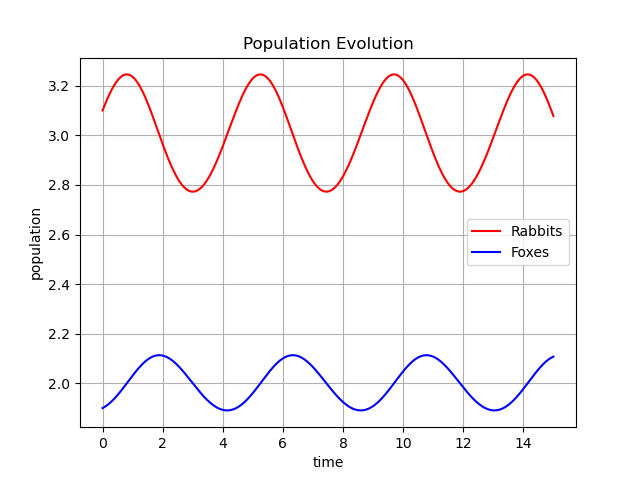
\includegraphics[scale=0.5]{images/2024-06-05-pred_prey_30.png}
    \end{subfigure}
    \begin{subfigure}{0.5\textwidth}
        \centering
        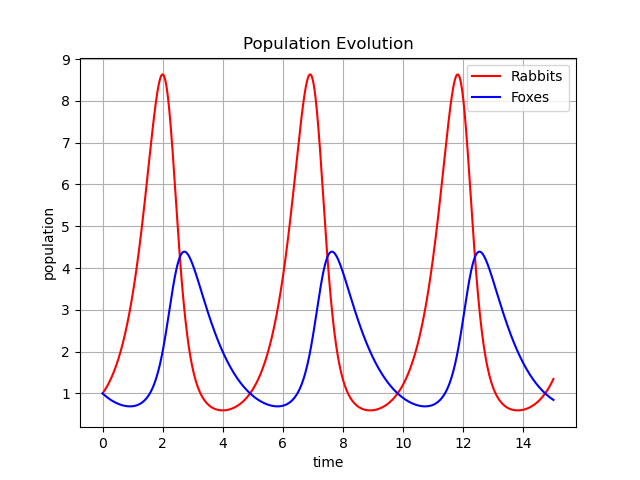
\includegraphics[scale=0.5]{images/2024-06-05-pred_prey_31.png}
    \end{subfigure}
\end{figure}


%%% Local Variables:
%%% mode: latex
%%% TeX-master: "journal"
%%% End:
